\chapter{Intermediate Testing and Reassessment}

This chapter discusses the methodology and learnings of our intermediate ground station testing, and how we used this data to shape our next steps for correlative assessment techniques.

\section{Testing}

Hakuto carried out a number of field tests on the ground station software previously described, including FDIR-related and correlative components. The major tests we conducted are described in detail below.

\subsection{Field Testing}

Over the course of two weeks, we performed daily field tests in the Lafarge rock quarry, located outside of Pittsburgh, Pennsylvania, USA, to both assess the physical characteristics of our radio communication and to confirm our mobility in a simulated lunar environment. (See Fig.~\ref{fig:night_test_team} for an image of the quarry terrain.) The ground station interface was in constant use throughout the course of the tests, with alternating drivers at the helm. The setup usually involved one primary pilot and one copilot, who helped with troubleshooting. See Fig.~\ref{fig:daytime_operation_pittsburgh_field_test} for an image of normal operation.

Our radio testing was multi-pronged. First, we endeavored to establish that we could communicate from the ground station to Moonraker and vice-versa by going through Astrobotic's radio relay, which we set up to emulate the lunar lander of our partner company, Astrobotic, which will function as a communication relay during the actual, planned lunar mission. Second, we tested the communication capabilities of Moonraker's radio antenna at two different operating frequencies (900 MHz and 2.4 GHz), in order to characterize performance over long distance and with line-of-sight blocked by rocky terrain. We looked for communication signal strength and commanding reliability in the presence of packet loss, and also tested the effect of a signal strength amplifier in a poor connectivity situation. These results were promising and are currently being analyzed by our communications team.

Our mobility testing consisted of driving long distances over rocky, yet generally even, terrain, often relying on our streaming video telemetry as visual feedback (instead of viewing the rover directly). We set up various challenges, such as large rock obstacles and inclines of increasing steepness, to test the rover's mobility capabilities as well as our operational capabilities using the ground station interface.

Other tasks performed during the field tests included coordinating with Hakuto crew and Astrobotic/Caltech engineers to fulfill mission tasks, scouting for field test locations, setting up and testing the ground station and radio equipment, and driving the rover during all of the tests to accomplish our test goals.

\begin{figure}[h]
\centering
    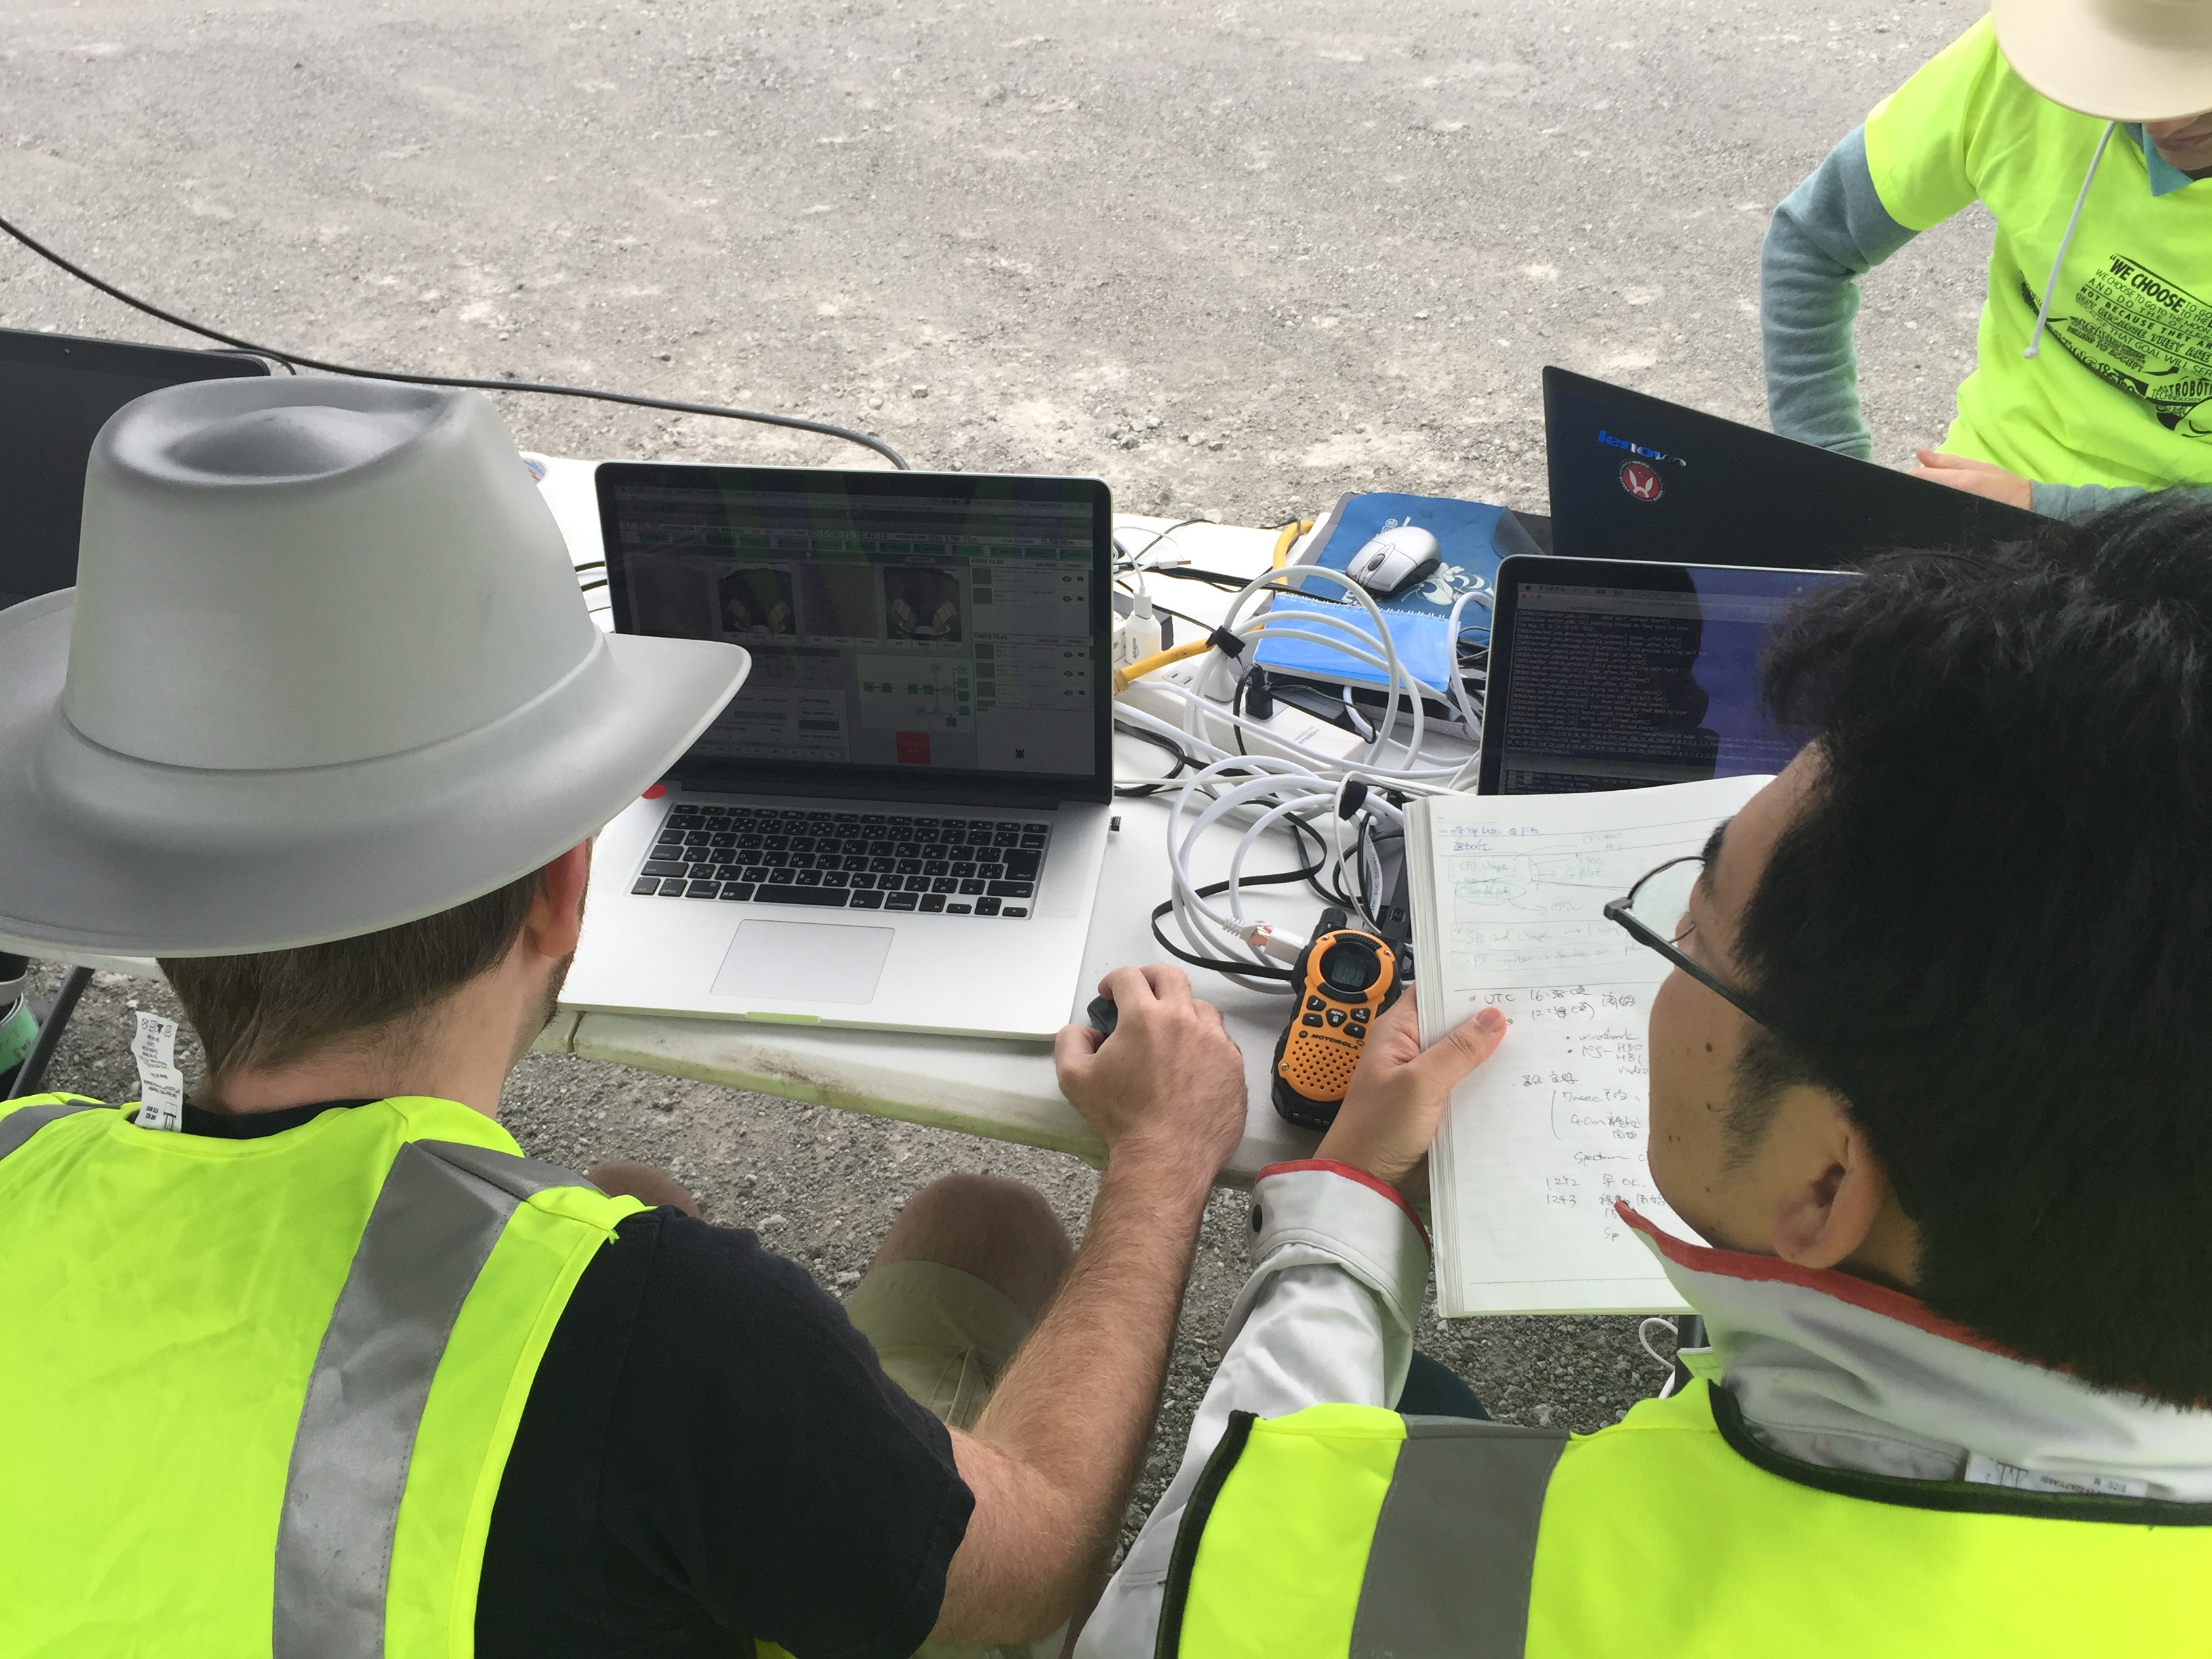
\includegraphics[width=\columnwidth]{images/daytime_operation_pittsburgh_field_test.jpg}
    \caption{Lead software engineer Toshiro Shimizu (right) and the author (left) work on radio testing during a field test at the Lafarge rock quarry.}
    \label{fig:daytime_operation_pittsburgh_field_test}
\end{figure}

\begin{figure}[h]
\centering
    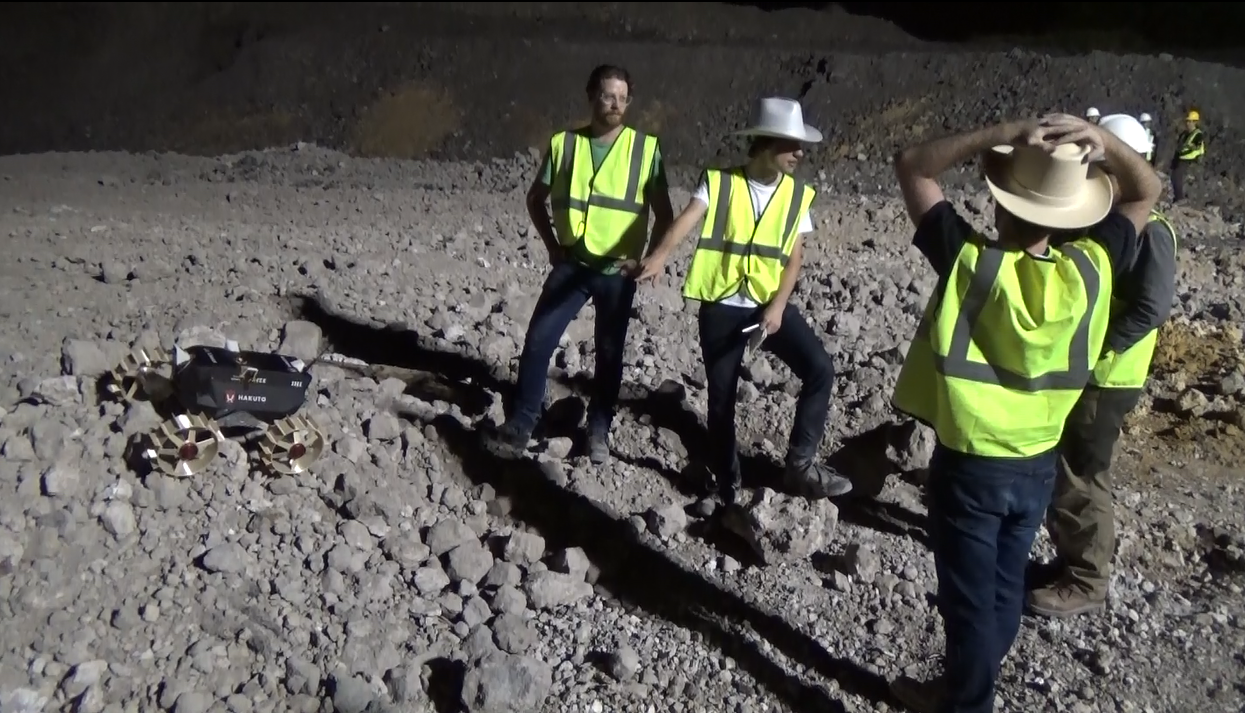
\includegraphics[width=\columnwidth]{images/night_test_team.png}
    \caption{Engineering members of Team Hakuto discuss terrain challenges during a nighttime field test.}
    \label{fig:night_test_team}
\end{figure}

\subsection{Field Test Results}

Our field tests went swimmingly, and we returned to Japan with excellent results and ideas for improvement, but these tests were not without a small number of issues. We uncovered several minor bugs within the ground station, which were quickly fixed on-the-spot. The tests---especially the act of watching others operate the ground station---yielded useful data about which features were used the most, and which were all but ignored entirely.

We found the ``immersive viewing" feature to be immensely helpful for gaining situational awareness, and proved its efficacy in a test in which engineers placed the rover in a precarious situation, then asked us over radio to use the telemetry and visual data to give them a detailed description of the current situation. The ``connectivity map" also proved extremely useful in quickly informing us of issues with the rover, as did the overall fault detection system. Some features were determined to be of limited utility and removed.

The ``Expert fault information" was shown to be somewhat inadequate in its coverage of expert understanding of problems, and there were several instances of users accidentally ignoring unsafe rover conditions. In response to these observations, space made available from removing other features was used for providing more detailed fault information. Also, fault detection and display rules were rethought and tweaked, to enhance visibility of anomalous states.

\subsection{Usability Testing}

In November 2015, we performed a set of usability tests on a slimmed-down version of the Moonraker ground station interface, in order to evaluate the various data analysis affordances and to determine any usability issues in need of attention. Seven users participated in the test, mostly interns and students possessing some familiarity with the rover, but with limited to no experience operating it via the ground station interface. See Fig.~\ref{fig:ui_test_takako} for an image of a user taking the test.

\begin{figure}[h]
\centering
    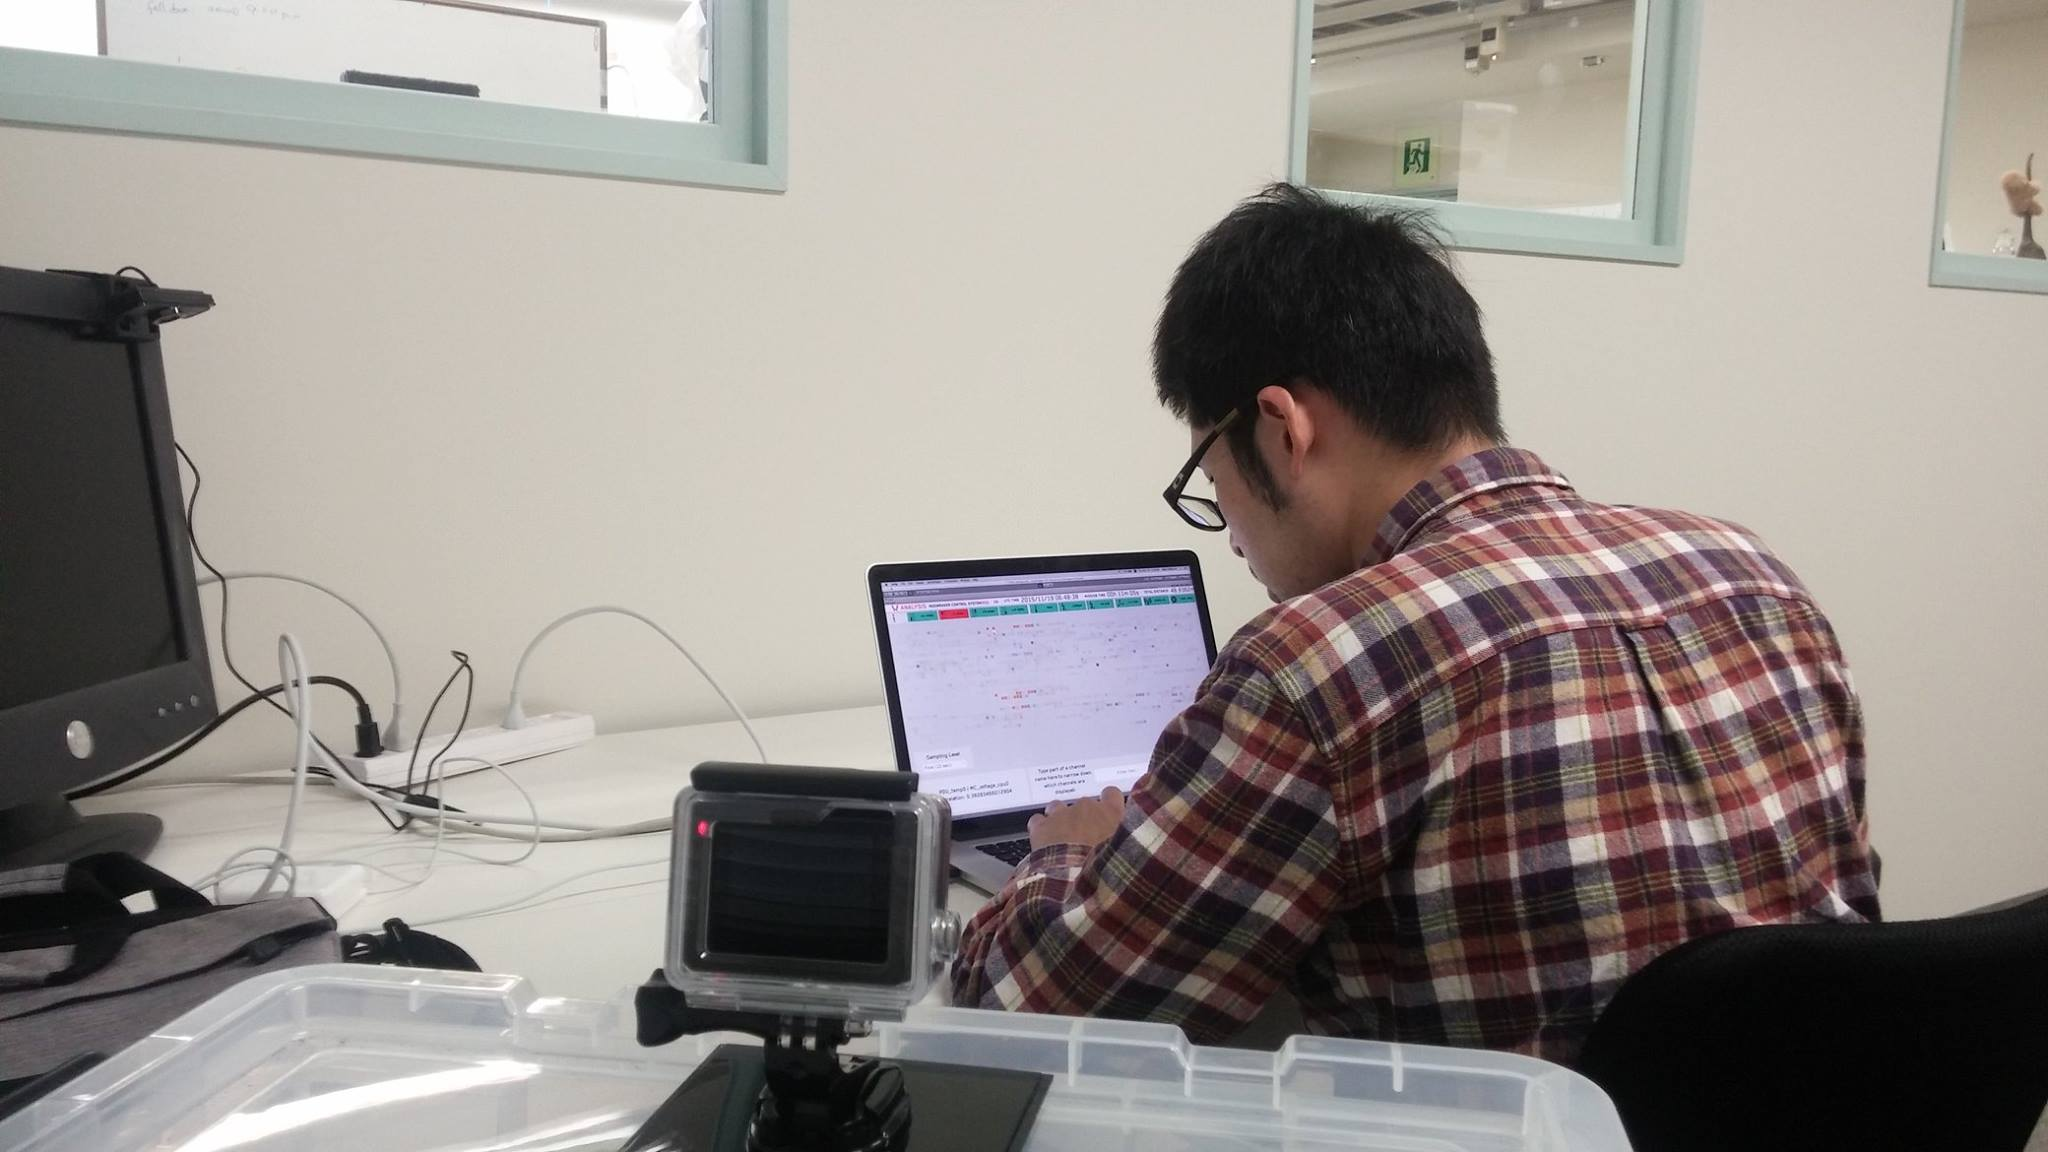
\includegraphics[width=\columnwidth]{images/ui_test_takuto.jpg}
    \caption{A usability test participant focuses on the incoming telemetry to try to ascertain patterns behind a faulted system.}
    \label{fig:ui_test_takako}
\end{figure}

Participants were presented with a simplified version of the ground station, with the Pilot Screen, Copilot Screen, and the Correlation Map screen. As the correlation map is a relatively novel idea, and has not (to the best of the author's knowledge) ever been used in ground station software, this test also served to see if it could be immediately usable in its present state, or if special training or modifications will be necessary before this visualization is useful for correlation discovery and root cause analysis.

\subsubsection{Test Tasks}

During the test, participants monitored telemetry and looked for patterns in received data during a $\sim$10-minute simulated drive on the lunar surface. During the course of the drive, camera images were unavailable, but the rover telemetry was indicative of various events that occurred to the rover during the run. The scenario consisted of the rover descending down into a crater, where it loses direct sunlight, resulting in reduced temperatures and solar charge voltages. It also loses line of sight with the lunar lander, causing packet losses and a reduction in signal strength. The rover then climbs out of the crater, bringing about an all-around improvement in these conditions. It enters some rough terrain, and ultimately stops after a rock becomes stuck in the wheel.

It was the task of the usability test participants to analyze the telemetry as it was received in order to try to understand the details of the story above. After the 10-minute run was complete, users were then given up to an additional 10 minutes to review received telemetry until they were satisfied they had understood the ``story" of the rover's trip. See Appendix~\ref{appendix:usability_test} for more detailed information about this test.

\subsection{Usability Test Results}

Usability testing yielded many results that were useful for setting subsequent development priorities.

We anticipated that users would be able to use the ground station tools to deduce the general course of events undergone by the rover, and this proved to be the case. Users' remarks showed that they understood the telemetry as displayed, and their intuition about the course of events matched the simulation plan closely. At the end of the test, each user was able to successfully narrate a story which resembled the intended one.

For example, as the simulated rover's telemetry began to show evidence of rough terrain, one user commented, ``we almost flipped... we're facing some harsh environment... probably passing through some rocks and obstacles." Some observations differed slightly from the details of the simulation, but matched the essence; when the simulated rover entered the shadow of the crater and its solar panel voltage began to drop, a user commented, ``maybe we're entering some sort of cave... because the solar panels... don't have enough energy."

Users remarked that they found the Copilot Screen's telemetry display the most useful, and they spent the majority of their time monitoring telemetry data on this screen. Most participants used the data review feature heavily while on this screen, rewinding and fast-forwarding through time and watching displayed telemetry values change as they did so. Users remarked that this feature was easy to use and excellent for reviewing the flow of telemetry. However, multiple users expressed a desire for time series plots of data channels, to better see the history of data at a glance.

Faults were generally very visible, and users commented that they found the additional fault information very helpful when trying to understand the meanings of various fault states. However, it was observed that tunnel vision was occasionally a problem for users; too much attention on one specific UI component, such as the correlation map or displayed telemetry on the Copilot Screen, seemed to be responsible for delays of up to 30 seconds in reacting to critical fault events. This observation led to the addition of audio cues to redirect user attention, which have already shown to be effective in informal testing.

Multiple users commented on the difficulty of understanding telemetry for channels whose meaning they did not understand. (Many of the subsystems have very specific data channels whose meaning is not well understood to anyone except the designers of those systems.) Results indicate that the expert fault information feature mentioned above was effective in eliminating much of the confusion about specific faults; however, we believe that adding information that leads to a better understanding of individual telemetry channels would result in less user confusion and could improve the effectiveness of human telemetry monitoring. Knowledge capture efforts are currently underway to collect detailed information about data channels from subsystem engineers to incorporate this data into the interface.

We hypothesized that users would find the correlation map to be a useful guide to seeing patterns in the data; however, our testing uncovered many issues with this visualization in its current form. Many of the users commented that they did not understand the proper way to use it to analyze data (although they understood the basic idea of the visualization). One user commented: ``It's difficult to pinpoint what we want to see." Users requested better, more intuitive spatial organization of data channel pairs, and the ability to more easily filter channels of interest and ones pertaining to faults. We received comments that additional training sessions might be beneficial. Nearly all users expressed an interest in using this feature, but the performance of those who endeavored to analyze faults with this tool showed evidence of a need for automated simplification to reduce stimuli, and to come up with better ways to train users and to lead them to useful conclusions. This motivated our desire to build followup visualizations capable of giving insight into correlative relationships, while minimizing cognitive load.

A few other minor issues came up which we had not foreseen until performing the testing. Some users had difficulties with transition lag between screens (there is a lag of approximately a second between screen transitions due to a need to load resources). We are looking into performance enhancements and/or loading screens to fix this issue. We also received the feedback that a more visible speed/RPM indicator for the rover would be helpful, as speed is one of the most important aspects of the rover as it operates, and this data is easily overlooked in the midst of other types of telemetry. This led to the development of the visual tachometer RPM visualization discussed in the previous chapter.

\section{Improvements and Additions}

Looking at the results of this intermediate testing, we were able to identify various targets for further research and improvements for analysis and visualization of the fault-related and correlative data.

Even with the small number of data channels available on the Moonraker rover ($\sim$112), the dimensionality was very high for a full corrgram display, and seemed to stretch the visual and attentive capacities of the users who participated in the test. Even with the addition of data filtering features, without training focused on the use of these features, they didn't seem to provide a better experience for users looking for patterns in the correlative data. Although users were, from an integrative viewing of telemetry data as shown in the numerical and color-based fault displays, able to come to understand a timeline of the rover events, mental links between associated channels seemed to emerge due to sheer coincidence; remarks from users were along the lines of ``the temperature is increasing... and I see that the voltage is increasing too... maybe they're related." The correlation map, as a way to call out these patterns, did not seem to be as effective as anticipated.

While the correlation data was successfully captured by our analysis, we determined that the ``important" correlations were buried in the noise of lots of unimportant ones, and shown on a larger visual display with too much data for a human to easily perceive in a short amount of time. What's more, there was no affordance for users to simultaneously display state data across different temporal points.

As such, we determined that it would be of value to iterate on these three points, with the main goals of reducing correlative noise and data dimensionality and of providing a simplified visualization capable of displaying data from multiple time points simultaneously. The next chapter will discuss a few approaches towards this end and their results.